\chapter{Automation}

Gravwell provides several utilities to enable automated operations.
Users can schedule searches to be executed at specific times, for
example every morning at 1:00. They can also schedule search
\emph{scripts}, which can execute multiple searches, sift and parse search
results, and send notifications via email or HTTP. These scheduled
operations are run by the \textbf{search agent}, a separate program which
connects to the Gravwell webserver as a client. This chapter describes
the search agent, scheduled searches, and scheduled scripts.

\section{Configuring User Email Settings}

In order to send emails from scheduled scripts, each user must input
settings for their preferred email server. This will allow Gravwell to
act as an SMTP client and send emails on the user's behalf. The email
configuration page is a sub-tab in the user's account settings (see Figure \ref{fig:email-prefs}).

\begin{figure}
	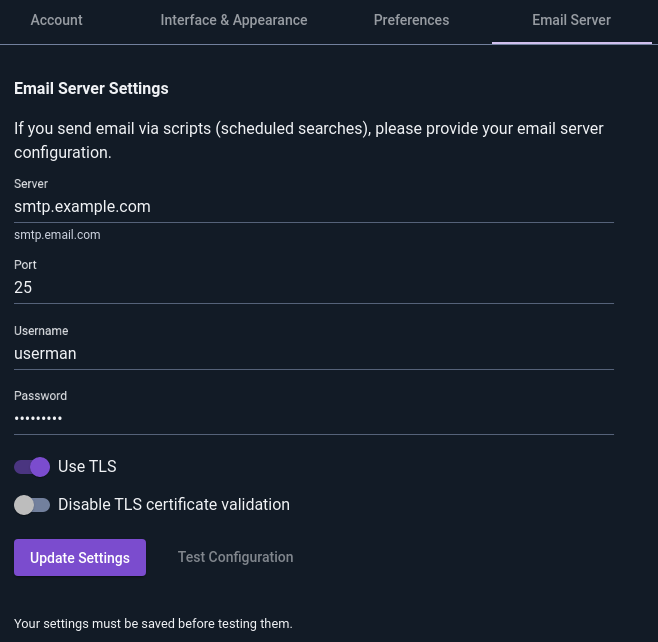
\includegraphics[width=0.7\linewidth]{images/email-prefs.png}
	\caption{Email preferences dialog}
	\label{fig:email-prefs}
\end{figure}

The Username and Password fields should be filled out with the user's
authentication tokens for the \emph{email server}. If TLS is required by
the server, set the `Use TLS' toggle; note that it may be necessary to
change the Port to 465 after enabling TLS.

After populating the configuration, hit `Update Settings' to save the
options. `Test Configuration' should then become clickable. Click it to
bring up the email testing
dialog, as seen in Figure \ref{fig:email-testing}.

\begin{figure}
	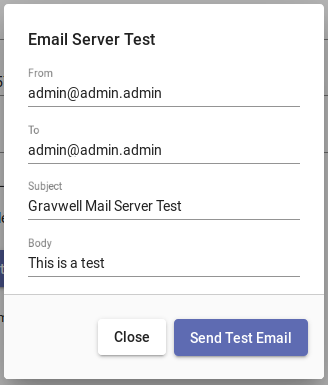
\includegraphics[width=0.5\linewidth]{images/email-testing.png}
	\caption{Email testing dialog}
	\label{fig:email-testing}
\end{figure}

Change the ``From'' and ``To'' addresses to the user's own email
address, then click `Send Test Email'. Gravwell will attempt to use the
mail server to send an email to the user. If the email arrives, the
email server has been correctly configured. It may be necessary to check
spam folders.

If the email does not arrive, check the Gravwell webserver logs,
located in \code{/opt/gravwell/log/web} by default.


\section{The Search Agent}

The search agent is the Gravwell component which actually handles the
execution of scheduled searches and scripts. It is a separate process
which connects to a Gravwell webserver as a client, obtains a list of
scheduled searches/scripts, and runs them when scheduled.

The search agent is shipped in the main Gravwell installer and should
be installed by default in most situations. If for some reason the
search agent is not enabled, a notification will appear in the Gravwell
web interface warning of that fact (Figure \ref{fig:searchagent-warn}).

\begin{figure}
	
\includegraphics[width=0.4\linewidth]{images/searchagent-warn.png}
	\caption{Search agent warning}
	\label{fig:searchagent-warn}
\end{figure}

Note that when using multiple Gravwell webservers, the search agent
should be disabled on all but one of them to avoid conflicts and
superfluous search executions.

\subsection{Disabling the Search Agent}

To disable the search agent on a server that uses Systemd:

\begin{Verbatim}[breaklines=true]
systemctl stop gravwell_searchagent.service
systemctl disable gravwell_searchagent.service
\end{Verbatim}

The Docker images provided by Gravwell do not use Systemd; instead,
they use a Gravwell-implemented process manager called ``manager''\footnote{https://github.com/gravwell/manager}. To disable the search agent on such a
container, pass the argument \code{-e DISABLE\_SEARCHAGENT=TRUE} when
creating the container, e.g.:

\begin{Verbatim}[breaklines=true]
docker run --rm --net gravnet -p 8080:80 -d \
-e DISABLE_SEARCHAGENT=TRUE --name gravwell gravwell:base
\end{Verbatim}

\subsection{Search Agent Configuration}

Although the search agent ships with the indexer and webserver
components, it uses its own configuration file found at
\code{/opt/gravwell/etc/searchagent.conf}. While the defaults set at
install time should be sufficient, this section describes the
configuration options in case changes are needed.

\subsubsection{Webserver-Address}

The \code{Webserver-Address} parameter should be an IP or hostname and a
port which point to the Gravwell webserver. If no port is specified,
port 443 is used by default (80 if HTTPS is disabled). The following are
all valid Webserver-Address values:

\begin{Verbatim}[breaklines=true]
Webserver-Address=10.0.0.1:80
Webserver-Address=127.0.0.1:443
Webserver-Address=192.168.0.1
Webserver-Address=gravwell-webserver.example.com
\end{Verbatim}

If Webserver-Address is specified multiple times, the search agent will multiplex
scheduled searches across all listed servers, to distribute load.

\subsubsection{Search-Agent-Auth}

The \code{Search-Agent-Auth} parameter specifies the token which is used to
authenticate with the webserver. This can be any string, but it
\emph{must} correspond with the \code{Search-Agent-Auth} parameter defined in
the webserver's \code{gravwell.conf}!

\subsubsection{Insecure-Use-HTTP}

Setting the \code{Insecure-Use-HTTP} parameter to ``true'' instructs the
search agent to connect to the Gravwell webserver using unencrypted
HTTP. This should only be used on trusted internal networks or on the
local loopback interface!

\subsubsection{Insecure-Skip-TLS-Verify}

Setting the \code{Insecure-Skip-TLS-Verify} parameter to true instructs
the search agent to ignore invalid TLS certificates when connecting to
the webserver.

\subsubsection{Log-File}

\code{Log-File} specifies a file where the search agent should write its
logs. If not set, the search agent will write logs to standard error.

\subsubsection{Log-Level}

\code{Log-Level} sets the severity level at which log entries will actually be
written to the log, thus setting \code{Log-Level=WARN} ensures only warnings,
errors, and critical messages will be sent to the log. The available
levels are OFF, DEBUG, INFO, WARN, ERROR, and CRITICAL.

\subsubsection{Max-Script-Run-Time}

The \code{Max-Script-Run-Time} parameter specifies how long, in minutes, a
given scheduled script is allowed to execute. If set to 0, scripts can
run for an unlimited length of time. There are two things to consider
when setting this:

\begin{enumerate}
\tightlist
\item
  A script which runs indefinitely only interferes with itself; other
  scheduled searches and scripts will run regardless.
\item
  Many buggy scripts will automatically time out, because a script must
  also execute at least one of the Gravwell-defined
  scripting functions every 30 seconds. A hung script will quickly
  be terminated.
\end{enumerate}


\subsection{Scheduling Searches}

Users can schedule searches to run at regular intervals. This enables
several useful possibilities, such as automatically updating lookup
tables (e.g. MAC address to IP mappings) or executing a very detailed /
long-running search every morning at 6 a.m. to have the results ready
when employees arrive.

\subsubsection{Creating a Scheduled Search}

To create a scheduled search, select the `Scheduled Searches' page from
the menu in the GUI, then click the `Add' button in the upper right
corner of the page. A form will pop up, as shown in Figure \ref{fig:new-scheduled}.

\begin{figure}
	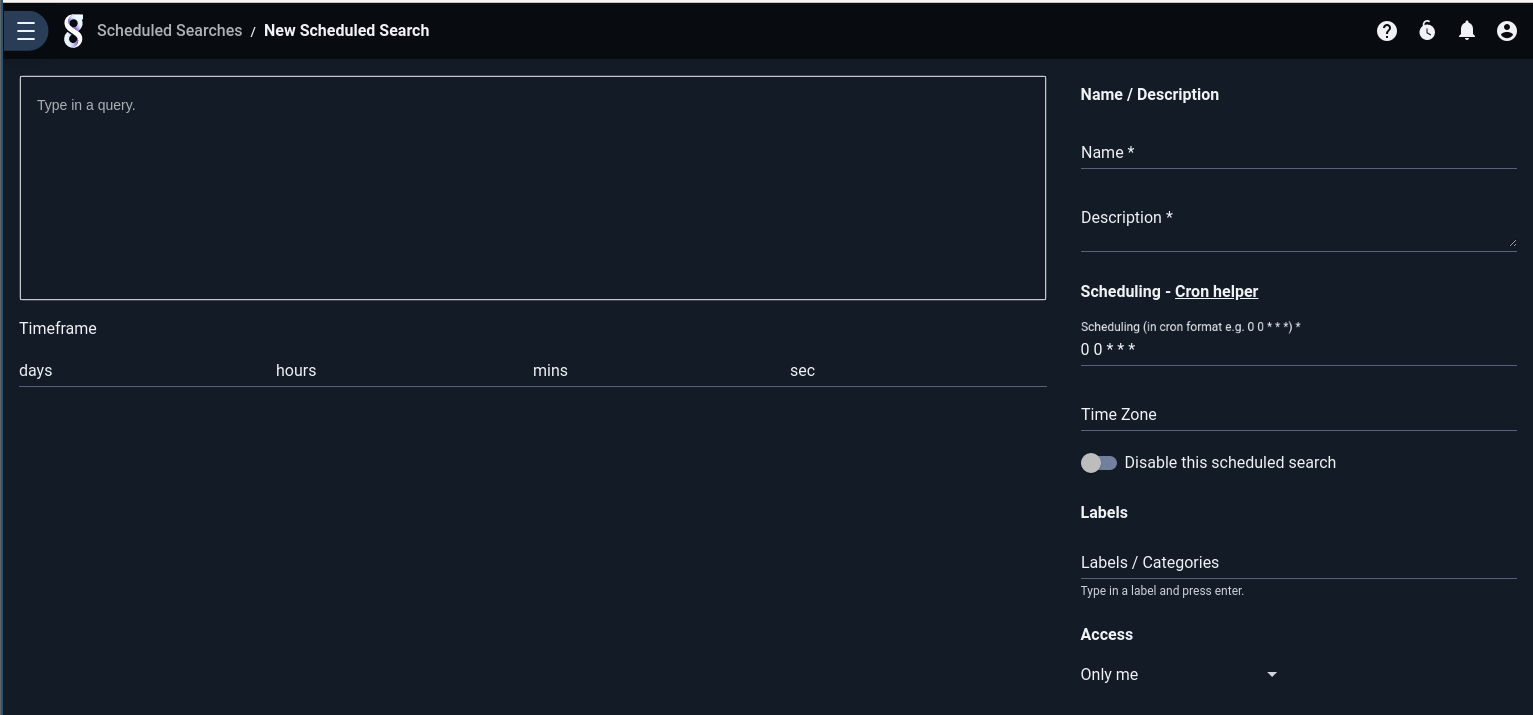
\includegraphics{images/new-scheduled.png}
	\caption{New scheduled search form}
	\label{fig:new-scheduled}
\end{figure}

Enter the desired query in the box labeled `Type in a query', then use
the timeframe picker to choose how far back the search should run.
Assign the scheduled search a name and a description.

The `Scheduling' field requires some explanation. This field defines a
cron-formatted schedule to specify when the search should run. Clicking
the `Cron Helper' link will open a useful website to experiment with
cron schedules. The following are all valid schedules:

\begin{itemize}
\tightlist
\item
  Run every minute: \code{* * * * *}
\item
  Run every 10 minutes: \code{*/10 * * * *}
\item
  Run every hour: \code{0 * * * *}
\item
  Run every day at 2 a.m.: \code{0 2 * * *}
\item
  Run once a week at 7 P.M.: \code{0 19 */7 * *}
\end{itemize}

When all the fields have been populated, click `Save' to save the
scheduled search. The search agent will soon discover this new search
and will execute it on schedule.

\subsubsection{Viewing Scheduled Search Results}

Once a scheduled search has been executed at least once, the results of
the most recent search execution are available for review. Although the
search results appear in the `Persistent Searches' page, the simplest
way to view the results for a particular scheduled search is to select
the `Run last search' icon on the tile for that scheduled search within
the `Scheduled Searches' page (Figure \ref{fig:run-last-search}).

\begin{figure}
	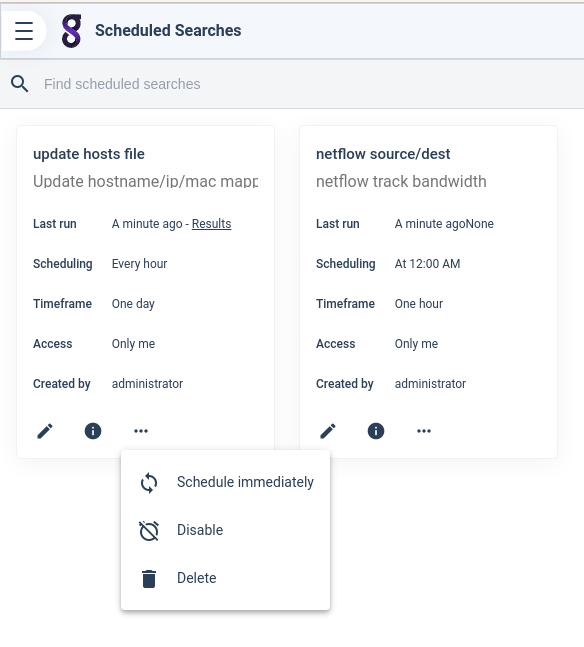
\includegraphics{images/run-last-search.png}
	\caption{The ``Run last search'' button}
	\label{fig:run-last-search}
\end{figure}

This will open the most recent results from that scheduled search. Note
that when the search agent runs a scheduled search, it deletes the
previous run's results when the new search completes. This prevents old
searches from cluttering the disk.

\subsection{Hands-On Lab}

This lab will demonstrate how a scheduled search can automatically
update lookup tables. First, create a Gravwell webserver+indexer
container:

\begin{Verbatim}[breaklines=true]
docker run -d --rm --net gravnet -p 8080:80 --name gravwell gravwell:base
\end{Verbatim}

Then we'll use the ingesters container (make sure you've loaded the ingesters container image as described in Section \ref{sec:load-lab-images}) to import some DHCP data:

\begin{Verbatim}[breaklines=true]
cd ~/gravwell_training/Automation/Lab-Scheduled

docker run -v $PWD/data:/tmp/data --rm -i --net gravnet \
gravwell:ingesters /opt/gravwell/bin/reimport -rebase-timestamp \
-clear-conns gravwell:4023 -i /tmp/data/dhcp.json.gz -import-format json \
-tag-override syslog
\end{Verbatim}

Log into the web GUI (\href{http://localhost:8080}{http://localhost:8080}).
 A simple search on the ``syslog'' tag over the last two weeks should show some results
similar to Figure \ref{fig:dhcp-data}.

\begin{figure}
	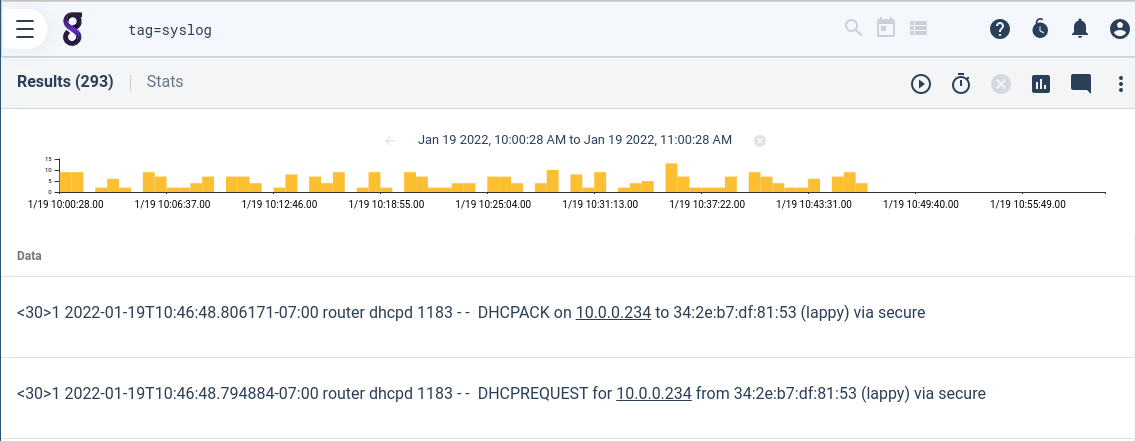
\includegraphics{images/dhcp-data.png}
	\caption{Raw DHPC logs}
	\label{fig:dhcp-data}
\end{figure}

These DHCP server logs can be used by a scheduled search to build a
lookup table for search enrichment, mapping MAC addresses and IP
addresses to hostnames. Go to the Scheduled Searches page, click `Add',
and fill in the form with the following:

\begin{itemize}
\item
  \textbf{Query:} 
\begin{Verbatim}[breaklines=true]
tag=syslog regex "HOSTNAME: (?P<hostname>\S+) on (?P<ip>\S+) at (?P<mac>\S+)" 
| unique hostname ip mac 
| table -save hosts hostname ip mac
\end{Verbatim}
\item
  \textbf{Timeframe:} \code{14 days}
\item
  \textbf{Name:} \code{hostsfile}
\item
  \textbf{Description:} \code{update hosts file}
\item
  \textbf{Scheduling:} \code{~* * * * *}
\end{itemize}

This scheduled search will run every minute, searching over the last 14
days to extract MAC:IP:hostname mappings. It will use the table
renderer's \code{-save} flag to save the results in a resource named
``hosts''.

Within a minute, a resource named ``hosts'' should appear on the
Resources page. We will test this lookup table by attempting to look up
the hostname which corresponds to the IP requested in DHCPREQUEST
messages. Here is a sample DHCPREQUEST message:

\code{\textless{}190\textgreater{} 11:15:02 apu dhcpd: DHCPREQUEST for
192.168.2.52 from 08:00:27:ca:b2:e7 via igb2}

From this, we can create a regular expression which extracts the IP
address, then use the new lookup table to match that IP address against
a hostname in the hosts resource. Figure \ref{fig:lookup-results} shows the
results.

\begin{Verbatim}[breaklines=true]
tag=syslog regex "DHCPREQUEST for (?P<ip>\S+)" 
| lookup -r hosts ip ip hostname as hostname | table
\end{Verbatim}

\begin{figure}
	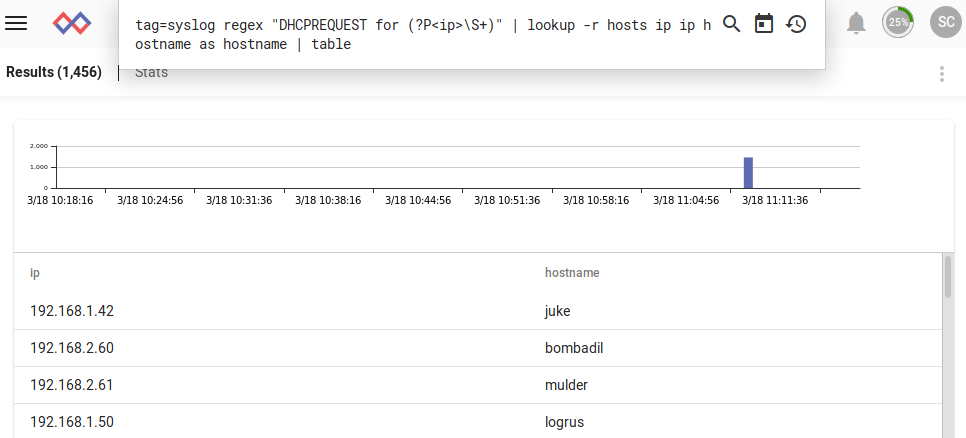
\includegraphics{images/lookup-results.png}
	\caption{Lookup table results}
	\label{fig:lookup-results}
\end{figure}

To clean up after the experiment, simply run:

\code{docker kill \$(docker ps -a -q)}

\section{Search Scripting and Orchestration}

Scripts provide an additional layer of power beyond scheduled
searches. A script can execute multiple searches, filter and enrich the
results, then re-ingest the resulting entries under a different tag,
send alerting emails, or do HTTP requests automatically.

Scripts can be run on a schedule, just like scheduled searches, or they
can be run manually with the command line client. This section will
first discuss how scripts are written, then delve into examples of how
they can be run and used.

A script can be scheduled in exactly the same way as a scheduled search
by simply changing the dropdown in the scheduled search creation form
from ``Search query'' to ``Anko script'' and pasting the script into the
form, as shown in Figure \ref{fig:create-soar}.

\begin{figure}
	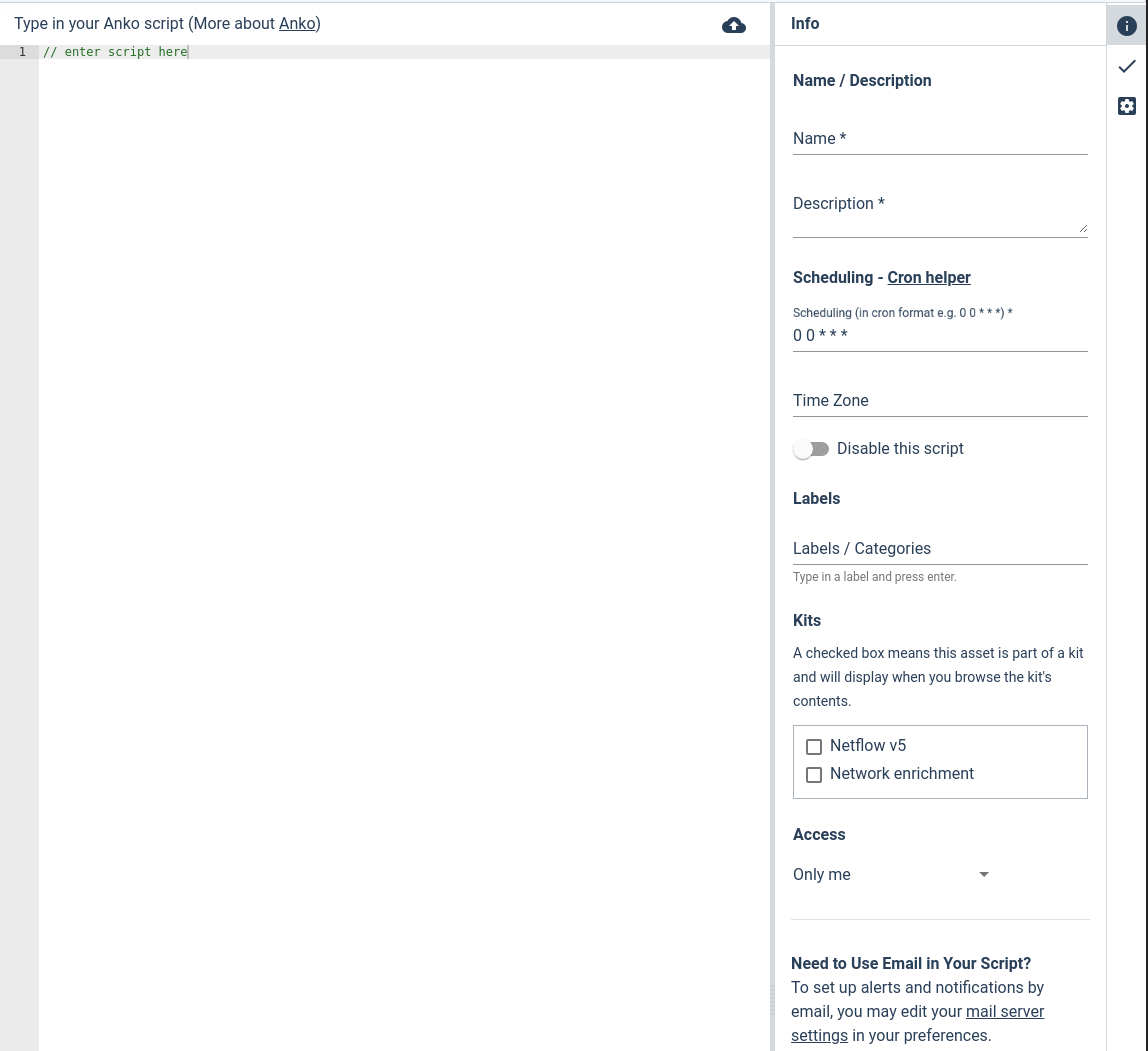
\includegraphics{images/create-soar.png}
	\caption{Creating a new scheduled script}
	\label{fig:create-soar}
\end{figure}

The rest of this section will describe what scripts look like and how
they are written.

\subsection{The Anko Scripting Language}

Gravwell scripts are written in the Anko scripting language (see
\href{http://github.com/mattn/anko}{http://github.com/mattn/anko}).
Anko is an interpreted, dynamically-typed language whose syntax
resembles Go. This section gives a brief overview of the language.

\subsubsection{Comments}

Anko comments can be prefixed with either the hash character or a pair
of slashes, or they can be wrapped in C-style comment markers:

\begin{Verbatim}[breaklines=true]
    // This is a valid Anko comment
    # This is also a valid comment
    /* This is a comment, too */
\end{Verbatim}

\subsubsection{Declaring variables}

In Anko, variables can be created and modified with the same syntax:

\begin{Verbatim}[breaklines=true]
    // This creates the variable
    x = 1
    // And this updates it
    x = x + 1
\end{Verbatim}


The `var' keyword can be used to indicate that a \emph{new} variable
\emph{must} be allocated at the current scope:

\begin{Verbatim}[breaklines=true]
    // Declare a variable
    var x = 1

    if true {
        // Declare a new variable at the inside scope
        var x = 2
    }
    println(x)    // prints “1”
\end{Verbatim}

If the `var' keyword was not used, the \code{println} call would have
printed `2'.

\subsubsection{Slices}

Anko implements slices (arrays) in a similar way to Go, but with more implicit
operations allowed:

\begin{Verbatim}[breaklines=true]
    a = [1, 2, 3]
    a += 4        // append
    println(a)    // prints [1 2 3 4]
    println(a[1])    // prints 2
\end{Verbatim}

Anko's default slice type is \code{[]interface\{\}}, which means a
slice can contain many different types. Note that slices are
``expanded'' when appended:

\begin{Verbatim}[breaklines=true]
    a = [1, 2.2, “foo”]
    a += [3, 4]
    a += [ [5, 6] ]
    println(a)    // prints [1 2.2 foo 3 4 [5 6]]
\end{Verbatim}


\subsubsection{Maps}

Anko maps are maps of \code{interface\{\}} to \code{interface\{\}}, meaning a
given map can mix key and value types:

\begin{Verbatim}[breaklines=true]
    m = { “foo”: 2 }    // initializes a map with a single entry, “foo” -> 2
    m[3] = 7        // map key 3 to value 7
    println(m[3])    // prints “7”
    println(m[“foo”]) // prints “2”
\end{Verbatim}


\subsubsection{If-Else Statements}

If-ElseIf-Else statements work exactly the same in Anko as in Go:

\begin{Verbatim}[breaklines=true]
    if x > 10 || y {
        count1++
    } else if x == 3 && !y {
        count2++
    } else {
        count3++
    }
\end{Verbatim}


\subsubsection{Switch Statements}

Anko provides switch statements similar to Go. Note that there is no
``fallthrough'' keyword.

\begin{Verbatim}[breaklines=true]
    switch val {
    case “foo”:
        count1++
    case 3:
        count2++
    default:
        notfound++
    }
\end{Verbatim}


\subsubsection{For Loops}

Anko supports traditional for loops:

\begin{Verbatim}[breaklines=true]
    for i = 0; i < 10; i++ {
      println(i)
    }
\end{Verbatim}

It also can also iterate over the contents of a slice:

\begin{Verbatim}[breaklines=true]
    a = ["foo", 3, 8.3]
    for i in a {
      println(i) // will print “foo”, 3, 8.3
    }
\end{Verbatim}

The `range' built-in function is convenient for iteration:

\begin{Verbatim}[breaklines=true]
    // this will print 0 through 9
    for i in range(0, 10) {
      println(i)
    }
    
    // this will print 0, 2, 4, 6, 8
    for i in range(0, 10, 2) {
      println(i)
    }
\end{Verbatim}

\subsubsection{Function Declaration}

Anko functions resemble Go functions, but they do not declare any
return types. Arguments are passed by value, not by reference:

\begin{Verbatim}[breaklines=true]
    func foo(x) {
      return x++
    }
    
    var a = 1
    foo(a)
    println(a)    // prints "1"
    a = foo(a)
    println(a)    // prints "2"
\end{Verbatim}

\subsection{Available Libraries}

A selection of Go libraries have some functionality exported to Anko for
use in scripts. Check the Gravwell online documentation for a full list.
Some examples are:

\begin{itemize}
\item ``bytes''
\item ``encoding/json''
\item ``errors''
\item ``math''
\item ``math/big''
\item ``math/rand''
\item ``net/url''
\item ``path''
\item ``path/filepath''
\item ``regexp''
\item ``sort''
\item ``strings''
\item ``time''
\item ``io''
\item ``flag''
\item ``io/ioutil''
\item ``encoding/csv''
\item ``crypto/md5''
\item ``crypto/sha1''
\item ``crypto/sha256''
\item ``crypto/sha512''
\item ``net''
\item ``net/http''
\item ``github.com/ziutek/telnet''
\item "google/uuid'' (github.com/google/uuid)
\end{itemize}

Libraries must be imported using the import function before use:

\begin{Verbatim}[breaklines=true]
    var md5 = import(“crypto/md5”)
    fooSum = md5.Sum(“foo”)
\end{Verbatim}

\subsection{Gravwell Anko Functions}

Gravwell has extended the Anko language with additional functions
specifically suited to writing orchestration scripts. This section
describes those functions. The functions are listed below in the format
\code{functionName(\textless{}functionArgs\textgreater{}) \textless{}returnValues\textgreater{}}.
Functions which return more than one argument have the return values wrapped in parentheses.

\subsubsection{Resources and persistent data functions}

``Persistent maps'' are a convenience offered for scheduled searches.
Values set in a persistent map will be available for reading in
subsequent runs of the scheduled search. If the named persistent map
does not exist, it will be created. Persistent maps do nothing when the
script is run at the Gravwell CLI.

\begin{itemize}
\tightlist
\item
  \code{getResource(name) ([]byte, error) } - returns the contents of the specified resource
  as a slice of bytes, while the error is any error encountered while fetching the resource.
\item
  \code{setResource(name, value) error} - creates (if necessary) and updates
  a resource named name with the contents of value, returning an error
  if one arises.
\item
  \code{setPersistentMap(mapname, key, value)} - stores a key-value pair
  in a map which will persist between executions of a scheduled script.
\item
  \code{getPersistentMap(mapname, key) value} - returns the value
  associated with the given key from the named persistent map.
\item
  \code{delPersistentMap(mapname, key)} - deletes the specified key/value
  pair from the given map.
\end{itemize}

\subsubsection{Search entry manipulation functions}

These functions get, set, and delete enumerated values on a single
entry (as returned by the \code{getEntries} function described later)

\begin{itemize}
\tightlist
\item
  \code{setEntryEnum(ent, key, value)} - sets an enumerated value on the
  specified entry.
\item
  \code{getEntryEnum(ent, key) (value, error)} - reads an enumerated value
  from the specified entry.
\item
  \code{delEntryEnum(ent, key)} - deletes the specified enumerated value
  from the given entry.
\end{itemize}

\subsubsection{General utility functions}

\begin{itemize}
\tightlist
\item
  \code{len(val) int} - returns the length of val, which can be a string,
  slice, etc.
\item
  \code{toIP(string) IP} - converts string to an IP, suitable for comparing
  against IPs generated by e.g. the packet module.
\item
  \code{toMAC(string) MAC} - converts string to a MAC address.
\item
  \code{toString(val) string} - converts val to a string.
\item
  \code{toInt(val) int64} - converts val to an integer if possible.
  Returns 0 if no conversion is possible.
\item
  \code{toFloat(val) float64} - converts val to a floating point number
  if possible. Returns 0.0 if no conversion is possible.
\item
  \code{toBool(val) bool} - attempts to convert val to a boolean.
  Returns false if no conversion is possible. Non-zero numbers and the
  strings ``y'', ``yes'', and ``true'' will return true.
\item
  \code{typeOf(val) type} - returns the type of val as a string, e.g.
  ``string'', ``bool''.
\end{itemize}

\subsubsection{Search management functions}

Due to the way Gravwell's search system works, some of the functions in
this section return Search structs (written as \code{``search''} in the
parameters) while others return search IDs (written as
\code{``searchID''} in the parameters). Each Search struct contains a
search ID, which can be accessed as \code{search.ID}.

Search structs are used to actively read entries from a search, while
search IDs tend to refer to inactive searches to which we may attach or
otherwise manage.

\begin{itemize}
\tightlist
\item
  \code{startBackgroundSearch(query, start, end) (search, err)} - creates
  a backgrounded search with the given query string, executed over the
  time range specified by 'start' and 'end'. The return value is a
  Search struct. These time values should be specified using the time
  library; see the examples for a demonstration.
\item
  \code{startSearch(query, start, end) (search, err)} - acts exactly like
  \code{startBackgroundSearch}, but does not background the search.
\item
  \code{detachSearch(search)} - detaches the given search (a Search
  struct). This will allow non-backgrounded searches to be automatically
  cleaned up and should be called whenever you're done with a search.
\item
  \code{attachSearch(searchID) (search, error)} - attaches to the search
  with the given ID and returns a Search struct which can be used to
  read entries etc.
\item
  \code{getSearchStatus(searchID) (string, error)} - returns the status of
  the specified search, which can be "ACTIVE", "ATTACHED", "DORMANT", "SAVED", "SAVING", or "UNKNOWN".
\item
  \code{getAvailableEntryCount(search) (uint64, bool, error)} - returns
  the number of entries that can be read from the given search, a
  boolean specifying if the search is complete, and an error if anything
  went wrong.
\item
  \code{getEntries(search, start, end) ([]SearchEntry, error)} - pulls
  the specified entries from the given search. The bounds for start and
  end can be found with the \code{getAvailableEntryCount} function.
\item
  \code{isSearchFinished(search) (bool, error)} - returns true if the
  given search is complete
\item
  \code{executeSearch(query, start, end) ({[}{]}SearchEntry, error)} -
  starts a search, waits for it to complete, retrieves up to ten
  thousand entries, \emph{detaches} from search and returns the entries.
\item
  \code{deleteSearch(searchID) error} - deletes the search with the
  specified ID
\item
  \code{backgroundSearch(searchID) error} - sends the specified search to
  the background; this is useful for ``keeping'' a search for later manual
  inspection.
\item
  \code{downloadSearch(searchID, format, start, end) ({[}{]}byte,
  error)} - downloads the given search as if a user had clicked the
  'Download' button in the web UI. \code{format} should be a string containing
  either ``json'', ``csv'', ``text'', ``pcap'', or ``lookupdata'' as appropriate.
  \code{start} and \code{end} are time values.
\item
  \code{getDownloadHandle(searchID, format, start, end) (io.Reader,
  error)} - returns a streaming handle to the results of the given
  search as if the user had clicked the 'Download' button in the web UI.
  The handle returned is suitable for use with the HTTP library
  functions shown later in this document.
\end{itemize}

\subsubsection{Search Data Type}

When executing a search via the \code{startSearch} or
\code{startBackgroundSearch} functions the \emph{search} data type is
returned. The search data type contains the following members:

\begin{itemize}
\tightlist
\item
  \code{ID} - A string containing the search ID. Use this member for other
  functions like \code{getSearchStatus} and \code{attachSearch}.
\item
  \code{RenderMod} - A string indicating the renderer attached to the
  search. It may be something like raw, text, table, chart, or fdg.
\item
  \code{SearchString} - A string containing the search string passed in
  during the request
\item
  \code{SearchStart} - A string containing the start timestamp for the
  search
\item
  \code{SearchEnd} - A string containing the end timestamp for the search
\item
  \code{Background} - A boolean indicating whether the search was started as
  a background search
\item
  \code{Name} - An optional string with a search name.
\end{itemize}

\subsubsection{Transmitting alerts or search results}

The scripting system provides several methods for transmitting script
results to external systems.

The following functions provide basic HTTP functionality:

\begin{itemize}
\tightlist
\item
  \code{httpGet(url) (string, error)} - performs an HTTP GET request on the
  given URL, returning the response body as a string.
\item
  \code{httpPost(url, contentType, data) (response, error)} - performs an
  HTTP POST request to the given URL with the specified content type
  (e.g. "application/json") and the given data as the POST body.
\end{itemize}

More elaborate HTTP operations are possible with the ``net/http''
library. See the package documentation in
the online anko
documentation\footnote{https://docs.gravwell.io/\#!scripting/scriptingsearch.md} for a description of what is available.

If the user has configured their personal email settings within
Gravwell, the email function is a very simple way to send an email:

\begin{itemize}
\tightlist
\item
  \code{email(from, to, subject, message) error} - sends an email via SMTP.
  The from field is simply a string, while to should be a slice of
  strings containing email addresses. The subject and message fields are
  also strings which should contain the subject line and body of the
  email.
\end{itemize}

\subsubsection{Creating and ingesting entries}

It is possible to ingest new entries into the indexers from within a
script using the following functions:

\begin{itemize}
\tightlist
\item
  \code{newEntry(time, data) Entry} - returns a new entry with the
  given timestamp (a \code{time.Time}, as from \code{time.Now()}) and
  \code{data} (frequently a string).
\item
  \code{ingestEntries(entries, tag) error} - ingests the given slice of
  entries (\code{[]Entry}) with the specified tag string.
\end{itemize}

The entries returned by the \code{getEntries} function can be modified if
desired and re-ingested via \code{ingestEntries}, or new entries can be created
from scratch. For example, to re-ingest some entries from a previous search
into the tag "newtag":

\begin{Verbatim}[breaklines=true]
    # Get the first 100 entries from the search
    ents, _ = getEntries(mySearch, 0, 100)
    ingestEntries(ents, "newtag")
\end{Verbatim}

To ingest new entries based on some other condition:

\begin{Verbatim}[breaklines=true]
    if condition == true {
        ents = make([]Entry)
        ents += newEntry(time.Now(), "Script condition triggered")
        ingestEntries(ents, "results")
    }
\end{Verbatim}

\subsection{Example Scripts}

This script creates a backgrounded search that finds which IPs have
communicated with Cloudflare's 1.1.1.1 DNS service over the last day. If
no results are found, the search is deleted, but if there are results
the search will remain for later perusal by the user in the `Persistent
Searches' screen of the GUI.


%%%%%%%%%%%%%%%%%%%%%%%%%%%%%%
% TODO: make sure this actually works
%%%%%%%%%%%%%%%%%%%%%%%%%%%%%%

\begin{Verbatim}[breaklines=true]
# Import the time library
var time = import("time")
# Define start and end times for the search
start = time.Now().Add(-24 * time.Hour)
end = time.Now()
# Launch the search
s, err = startSearch("tag=netflow netflow Dst==1.1.1.1 Src | unique Src | table Src", start, end)
if err != nil {
    return err
}
# Wait until the search is finished
for {
    f, err = isSearchFinished(s)
    if err != nil {
        return err
    }
    if f {
        break
    }
    time.Sleep(1 * time.Second)
}
# Find out how many entries were returned
c, _, err = getAvailableEntryCount(s)
if err != nil {
    return err
}
# If no entries returned, delete the search
# Otherwise, background it
if c == 0 {
    deleteSearch(s.ID)
} else {
    err = backgroundSearch(s.ID)
    if err != nil {
        return err
    }
}
# Always detach from the search at the end of execution
detachSearch(s)
\end{Verbatim}


%%%%%%%%%%%%%%%%%%%%%%%%%%%%%%
% TODO: update for the GUI
%%%%%%%%%%%%%%%%%%%%%%%%%%%%%%
\subsection{Developing \& Testing Scripts}

Because the same script can be executed as either a scheduled search or
manually with the CLI client, scripts are usually tested/developed using
the CLI client and then copied into a scheduled search later. Scripts
run with the CLI client can display printed output, which is ignored
when run on a schedule; this is particularly useful when debugging a
script.

A script can be executed manually from the client in the following
way:

\begin{Verbatim}[breaklines=true]
$ gravwell -s <server> script
script file path> /path/to/script.ank
\end{Verbatim}

A convenient way to run a script repeatedly is to use the ``watch''
modifier. The client will execute the script, then prompt to re-run. If
the script file is modified between runs, the next execution will use
the updated script. Here, a script that hashes a string with MD5 is
modified to hash using SHA1:

\begin{Verbatim}[breaklines=true]
$ gravwell -s <server> watch script
script file path>  /tmp/hash.ank
[172 189 24 219 76 194 248 92 237 239 101 79 204 196 164 216]
Hit [enter] to re-run, or [q][enter] to cancel

[11 238 199 181 234 63 15 219 201 93 13 212 127 60 91 194 117 218 138 51]
Hit [enter] to re-run, or [q][enter] to cancel
\end{Verbatim}


%%%%%%%%%%%%%%%%%%%%%%%%%%%%%%
% TODO: update for the GUI
%%%%%%%%%%%%%%%%%%%%%%%%%%%%%%
\subsection{Hands-on Lab: Scripting}

This lab will demonstrate how to send email alerts from a script. This
lab will test the script using the Gravwell CLI client, then schedule it
for automated execution.

The script will operate on Netflow records and send an alert whenever
traffic is seen originating from the 7.0.0.0/8 subnet, which in this
example stands in for a ``known bad'' subnet or subnets. In an actual
deployment, one might keep a list of known-bad subnets in a resource
lookup table (which can be automatically updated via another script!)
and compare flow records against that lookup table instead, but for
simplicity we will use a single hard-coded subnet.

First, launch a Gravwell webserver+indexer container:

\begin{Verbatim}[breaklines=true]
docker run --rm --net gravnet -p 8080:80 -d --name gravwell gravwell:base
\end{Verbatim}

Log in, go to the Account
settings page and select the Email Server tab, then populate your email
server configuration and test it (Figure \ref{fig:lab-emailsettings}).

\begin{figure}
	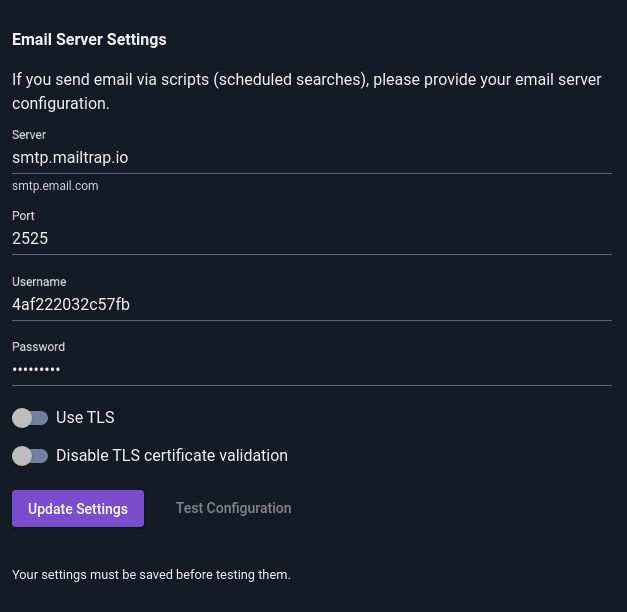
\includegraphics{images/lab-emailsettings.png}
	\caption{Configuring email server}
	\label{fig:lab-emailsettings}
\end{figure}

Next, start the ingester container running the Netflow ingester:

\begin{Verbatim}[breaklines=true]
docker run --rm -d --net gravnet --name ingesters \
-e GRAVWELL_CLEARTEXT_TARGETS=gravwell:4023 gravwell:ingesters \
/opt/gravwell/bin/gravwell_netflow_capture
\end{Verbatim}

The Netflow ingester is pre-configured to listen on port 2055 for
incoming Netflow v5 records.

Now, we use another Docker container to generate Netflow records and
send them to the ingester:

\begin{Verbatim}[breaklines=true]
docker run -it --net gravnet --rm \
networkstatic/nflow-generator -t ingesters -p 2055
\end{Verbatim}

The Netflow generator will run indefinitely, generating flow records,
until killed. Let it run at least until the following query shows at
least one result:

\begin{Verbatim}[breaklines=true]
tag=netflow netflow Src | subnet Src /8 as sub | ip sub == 7.0.0.0 | table
\end{Verbatim}

This query will form the basis of our script. It extracts the source IP
address from the Netflow records, converts that to a /8 subnet and
stores the result in an enumerated value named ``sub'', then compares
``sub'' to 7.0.0.0.

Open the file named \code{email-netflow.ank}  on the host system and paste
the following into it (or use the version in the training package):

\begin{Verbatim}[breaklines=true]
var time = import("time")
# SET THESE VARIABLES
from = "MY.ADDRESS@EXAMPLE.COM"
to = [ "RECIPIENT@EXAMPLE.COM" ]
my_name = "HANK"
# Do the search over the last day
end = time.Now()
start = end.Add(-24 * time.Hour)
query = `tag=netflow netflow Src | subnet Src /8 as sub | ip sub == 7.0.0.0 | table`
s, err = startSearch(query, start, end)
if err != nil {
        return err
}
# Wait for the search to complete
for {
        f, err = isSearchFinished(s)
        if err != nil {
                return err
        }
        if f {
                break
        }
        time.Sleep(1 * time.Second)
}
# Figure out how many results there were
c, _, err = getAvailableEntryCount(s)
if err != nil {
        return err
}
# clean up the search, we only care about how many entries there were
detachSearch(s)

# If there was more than 0 entries, send an email
if c > 0 {
        summary = "There were " + c + " flows originating from the banned subnet!"
        email(from, to, my_name + " alert!", summary)
}
\end{Verbatim}

Modify the \code{`from'}, \code{`to'}, and \code{`my\_name'} variables at the
top of the script; `from' should be your email address, `to' is a list
of email recipients (this should probably be your email address again),
and `my\_name' is your own name.

Now copy the file to the Gravwell container and run a shell:

\begin{Verbatim}[breaklines=true]
docker cp email-netflow.ank gravwell:/tmp/
docker exec -it gravwell /bin/sh
\end{Verbatim}

Within that shell, run the Gravwell CLI client and execute the script:

\begin{Verbatim}[breaklines=true]
$ gravwell -insecure-no-https script
script file path>  /tmp/email-netflow.ank
\end{Verbatim}

If all goes well, an email alert should arrive soon!

The script can be trivially run on a schedule by simply pasting it into
the New Scheduled Search dialog, as shown in Figure \ref{fig:lab-create-script}.

\begin{figure}
	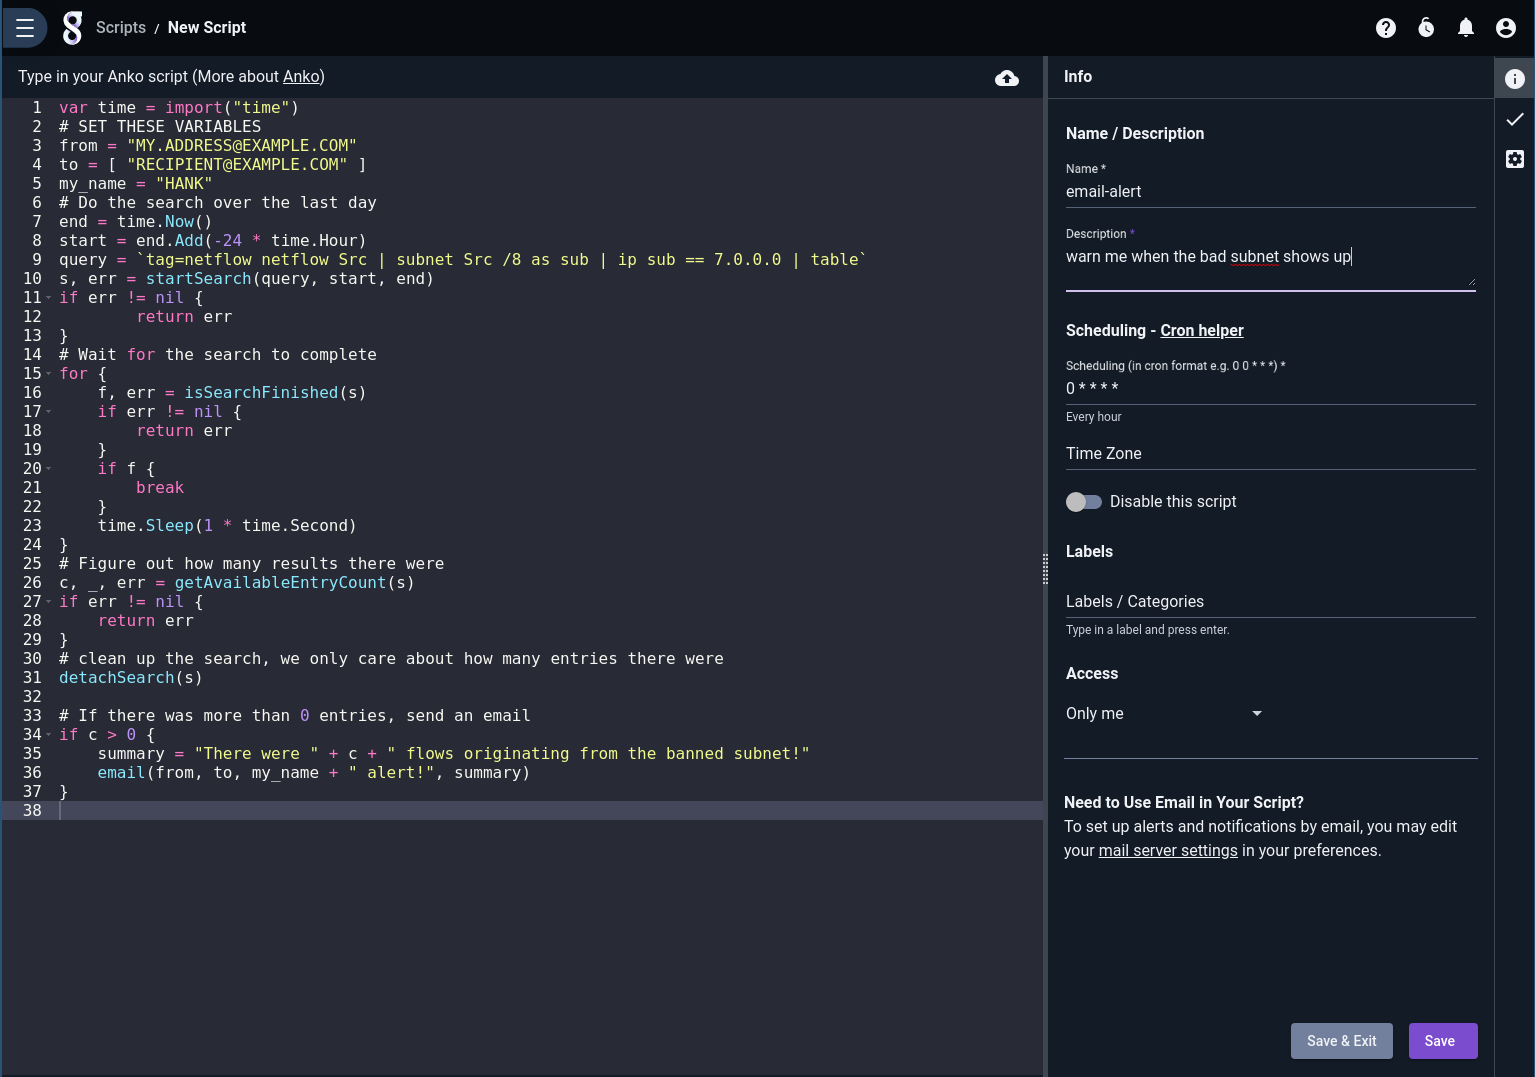
\includegraphics{images/lab-create-script.png}
	\caption{Creating scheduled script}
	\label{fig:lab-create-script}
\end{figure}

Note that this will send an email every minute, so either delete the
scheduled script once it's been verified to work, or shut down the
entire experiment when satisfied:

\code{docker kill \$(docker ps -a -q)}
